\documentclass[a4paper,10pt]{article}
\usepackage{epsfig}
\usepackage{latexsym}
\usepackage{graphicx}
\usepackage{amsfonts}
\usepackage{amsmath}
\usepackage{xcolor}

%-----------------------------------------
% Pour accepter les lettres accentuees de clavier azerty
% sans les \'e (utile) pour tapper directement en azerty 
% et ou faire passer aspell -c --lang=fr bidon.tex
%\usepackage[latin1]{inputenc}
%------------------------------------------


%\topmargin=-3cm
\topmargin=-1cm
\oddsidemargin=-1cm
\evensidemargin=-1cm
\textwidth=17cm
%\textheight=27cm
\textheight=25cm
\raggedbottom
\sloppy

\definecolor{Blue}{rgb}{0.,0.,1.}
\definecolor{LightSkyBlue}{rgb}{0.691,0.827,1.}
\definecolor{Red}{rgb}{1.,0.,0.}
\definecolor{Green}{rgb}{0.,1.,0.}
\definecolor{Purple}{rgb}{0.5, 0., 0.5}
\definecolor{Try}{rgb}{0.15,0.,1}
\definecolor{Black}{rgb}{0., 0., 0.}

%To get DRAFT accross all pages
%\usepackage{draftcopy}
%To replace ``DRAFT'' by ``ON GOING''
%\draftcopyName{ON GOING}{150}

\title{HWP parameters estimation}
\author{N.~Ponthieu, A.~Catalano}

\begin{document}
\maketitle
\tableofcontents

\begin{abstract}
Cette note a pour but de servir de r\'ef\'erence en mati\'ere de
notations et de d\'efinition des diff\'erents param\`etres
instrumentaux qui entrent dans les simulations de PILOT. Elle
commence par la d\'efinition des param\`etres de Stokes et
d\'ecrit leurs propri\'et\'es principales.
\end{abstract}

\section{Introduction : les Param\`{e}tres de Stockes}

\subsection{D\'efinition}

Le champ \'{e}lectrique d'une onde \'{e}lectromagn\'{e}tique est
d\'{e}fini par ses deux composantes $E_{x}$ et $E_{y}$ dans un
rep\`{e}re $(x,y)$ orthonormal \`{a} la direction de propagation
de l'onde $z$:

\begin{eqnarray}
E_x(t) & = & A_xe^{i\omega t} \nonumber \\
E_y(t) & = & A_ye^{i(\omega t+\phi)}
\end{eqnarray}

D\'{e}terminer la polarisation d'une onde revient donc \`{a}
d\'{e}terminer la valeur des param\`{e}tres $A_y$, $A_y$ et $\phi$
\`{a} chaque instant. En pratique il est possible de mesurer
uniquement les intensit\'{e}s $\langle |E_{x}^{2}|\rangle$ et
$\langle |E_{x}^{2}|\rangle$ d'un rayonnement compte-tenu de la
rapidit\'{e} d'oscillation des ondes lumineuses fix\'{e}e par
$\omega$. Les dur\'{e}s de moyennage associ\'{e}es aux
intensit\'{e}s mesur\'{e}es correspondent alors au temps
d'int\'{e}gration du d\'{e}tecteur. On d\'efinit alors les
\emph{param\`{e}tres de Stokes} $I$, $Q$ et $U$ par :

\begin{eqnarray}
I & = & \langle |E_{x}|^2\rangle+\langle|E_y|^2\rangle=I_x + I_y \\
Q & = & I_x-I_y \\
U & = & I_{x}^{45}-I_{y}^{45}
\end{eqnarray}

Le param\`{e}tre $U$ est calcul\'{e} \`{a} partir des composantes
du champ \'{e}lectrique de l'onde \'{e}tudi\'{e}e suivant deux
axes orthogonaux orient\'es \'{a} 45$^{\circ}$ du rep\`{e}re de
calcul de $I$ et $Q$. Le degr\'e de polarisation lin\'eaire $p$
est alors d\'efini par:

\begin{equation}
p = \frac{\sqrt{Q^2 + U^2}}{I}\label{degredepola}
\end{equation}

Une fois $I$, $Q$ et $U$ mesur\'{e}s, il est possible de remonter
\`{a} $A_{x}^{2}$, $B_{x}^{2}$ et $\phi$.  $I$ et $Q$ fournissent
$A_{x}^{2}$ et $B_{x}^{2}$, $U$ fournit $\phi$:

\begin{eqnarray}
U & = & I_{x}^{45}-I_{y}^{45}\nonumber\\
  & = & \langle|\frac{1}{\sqrt{2}}(E_{x}+E_{y})^{2}|\rangle-\langle
|\frac{1}{\sqrt{2}}(-E_{x}+E_{y})^{2}|\rangle\nonumber\\
  & = & \frac{1}{2}|A_{x}+A_{y}e^{i\phi}|^{2}
-\frac{1}{2}|-A_{x}+A_{y}e^{i\phi}|^{2}\nonumber \\
  & = & \frac{1}{2}|A_{x}+A_{y}\cos\phi+iA_{y}\sin\phi|^{2}-
\frac{1}{2}|-A_{x}+A_{y}\cos\phi+iA_{y}\sin\phi|^{2}=... \nonumber\\
U & = & 2A_{x}A_{y}\cos\phi
\end{eqnarray}

\subsection{Alg\`ebre des Param\`etres de Stokes}

Avant de relier les param\`etres $I, Q, U$ aux mesures d'un
d\'etecteur polaris\'e dans le paragraphe suivant, nous allons
tout d'abord montrer comment ils se transforment quand on change
la base de r\'ef\'erence. Nous supposons pour cela que dans la
base $(x, y)$ les param\`etres de l'onde sont $(I, Q, U)_{xy}$, et
que nous cherchons les param\`etres $(I, Q, U)_{ab}$ dans la base
$(a, b)$, o\`u la direction $a$ fait un angle $\alpha$ avec l'axe
$x$ (cf.~Fig.~\ref{change_orientation}).

\begin{figure}
\begin{center}
\includegraphics[scale=0.35,angle=0]{change_orient.eps}
\caption{\footnotesize Convention d'orientation relative des bases
$(x, y)$ et $(a, b)$ dans lesquelles on cherche les param\`etres
de Stokes de l'ellipse de polarisation repr\'esent\'ee.}
\label{change_orientation}
\end{center}
\end{figure}

L'intensit\'e est bien \'evidemment conserv\'ee. Nous avons alors
:

\begin{equation}
\left(\begin{array}{c}
E_a \\
E_b\end{array}\right) =\left(\begin{array}{rc}
\cos\alpha & \sin\alpha \\
-\sin\alpha & \cos\alpha \end{array}\right) \left(\begin{array}{c}
E_x \\
E_y\end{array}\right)
\label{eq:rot_basis_jones}
\end{equation}

Ainsi\footnote{Nous omettons volontairement le facteur
$e^{-i\omega t}$ pour ne pas alourdir les notations} :

\begin{eqnarray}
Q_{ab} & = & \langle |E_a|^2\rangle - \langle |E_b|^2\rangle
\nonumber
\\ & = & \vert \cos\alpha A_x + \sin\alpha A_ye^{i\phi}\vert^2 -
\vert-\sin\alpha A_x + \cos\alpha A_ye^{i\phi}\vert^2 \nonumber \\
& = & (A_x^2 - A_y^2)\, \cos2\alpha + 2A_xA_y\cos\phi \,
\sin2\alpha \nonumber \\ & = & Q_{xy}\, \cos2\alpha + U_{xy}\,
\sin2\alpha \nonumber
\end{eqnarray}

Le calcul est similaire pour $U_{ab}$ en faisant le changement
$\alpha \rightarrow \alpha + \pi/4$ :

\begin{center}
\begin{math}
U_{ab} = -Q_{xy}\, \sin2\alpha + U_{xy}\, \cos2\alpha
\end{math}
\end{center}

Nous pouvons donc \`a pr\'esent donner la relation g\'en\'erale de
transformation des param\`etres de Stokes dans une base $(a, b)$
dont l'axe $a$ fait l'angle $\alpha$ par rapport \`a l'axe $x$ de
la base d'origine :

\begin{eqnarray}
\left(\begin{array}{c}
I \\
Q \\
U \end{array}\right)_{ab} & = & \left(\begin{array}{crc}
1 & \cdot & \cdot \\
\cdot & \cos2\alpha & \sin2\alpha \\
\cdot & -\sin2\alpha & \cos2\alpha
\end{array}\right)
\left(\begin{array}{c}
I \\
Q \\
U \end{array}\right)_{xy} \label{eq:rot_basis}\\
& = & \mathcal{R}_{\alpha}\left(\begin{array}{c}
I \\
Q \\
U \end{array}\right)_{xy} \label{eq:rot_stokes}
\end{eqnarray}

La relation pr\'ec\'edente fournit imm\'ediatement la
d\'etermination de l'orientation de l'ellipse. En effet, dans la
base propre de l'ellipse, d\'efinie par son grand et son petit
axe, les param\`etres de Stokes sont : $Q_{propre} = pI$ et
$U_{propre}=0$. Si l'ellipse fait l'angle $\psi$ par rapport \`a
notre axe $x$ de r\'ef\'erence, l'application de la relation
(\ref{eq:rot_stokes}) pour l'angle $-\psi$ conduit \`a :

\begin{eqnarray}
Q & = & \cos2\psi \;Q_{propre} \label{eq:q_propre}\\
U & = & \sin2\psi \;Q_{propre} \label{eq:u_propre}
\end{eqnarray}

et donc

\begin{equation}
\psi =  \frac{1}{2}\arctan\frac{U}{Q}
\end{equation}

\textbf{Remarques :}

\begin{itemize}
\item On prendra garde dans le calcul de l'arctangente, \`a ne pas
prendre brutalement l'arctangente math\'ematique, d\'efini sur
$]-\frac{\pi}{2}, \frac{\pi}{2}[$, sinon l'angle $\psi$ se
retrouverait contraint dans $]-\frac{\pi}{4}, \frac{\pi}{4}[$. Il
faudra d\'eterminer l'angle $2\psi$ entre 0 et $2\pi$, pour bien
d\'eterminer ensuite $\psi$ qui est bien d\'efini \`a $\pi$
pr\`es.
\end{itemize}

\subsection{Lien entre les matrices de Mueller et les matrices de
Jones}
\label{se:jones2mueller}

Les matrices qui agissent sur les param\`etres de Stokes sont connues
sous le nom de matrice de Mueller, celles qui agissent sur les
composantes du champ \'electrique sous le nom de matrices de
Jones. Dans le cas de la mod\'elisation de l'effet de l'instrument sur
le rayonnement, il est parfois plus intuitif de se ref\'erer au
formalisme de Jones. Il est donc important de pouvoir faire le lien
entre les deux. Nous donnons ici les relations de base et quelques
exemples.\\

Si l'on num\'erote les matrices de Pauli de la fa\c con suivante (pas
usuelle):

\begin{equation}
\sigma_0 \equiv \left(\begin{array}{cc}
1 & 0\\
0 & 1\end{array}\right)\;\;\;\;\;
\sigma_1 \equiv \left(\begin{array}{cc}
1 & 0\\
0 & -1\end{array}\right)\;\;\;\;\;
\sigma_2 \equiv \left(\begin{array}{cc}
0 & 1\\
1 & 0\end{array}\right)\;\;\;\;\;
\sigma_3 \equiv \left(\begin{array}{cc}
0 & -i\\
i & 0\end{array}\right)
\end{equation}

alors si $k$ d\'esigne l'indice de ligne et $\l$ l'indice de colonne,
la matrice de Mueller s'obtient \`a partir de la matrice de Jones par:

\begin{eqnarray}
M_{kl} & = & \frac{1}{2}Tr\left(\sigma_k J \sigma_l J^\dag\right) \label{eq:jones2mueller_1}\\
&=& \frac{1}{2}\left(\begin{array}{rrr}
|J_{00}|^2 + |J_{01}|^2 + |J_{10}|^2 + |J_{11}|^2 &
|J_{00}|^2 - |J_{01}|^2 + |J_{10}|^2 - |J_{11}|^2 &
2Re(J_{00}J_{01} + J_{10}J_{11}) \\

|J_{00}|^2 + |J_{01}|^2 - |J_{10}|^2 - |J_{11}|^2 &
|J_{00}|^2 - |J_{01}|^2 - |J_{10}|^2 + |J_{11}|^2 &
2Re(J_{00}J_{01} - J_{10}J_{11}) \\

2Re( J_{00}J_{10} + J_{01}J_{11}) &
2Re( J_{00}J_{10} - J_{01}J_{11}) &
2Re( J_{00}J_{11} + J_{01}J_{10})\end{array}\right) \label{eq:jones2mueller_2}
\end{eqnarray}

o\`u $^\dag$ signifie transpos\'e et conjugu\'e. Ci-dessous quelques
exemples usuels.\\

{\bf Remarque:} Dans le cas le plus g\'en\'eral on doit consid\'erer
un quatri\`eme param\`etre de Stokes $V$, qui caract\'erise le degr\'e
de polarisation circulaire de l'onde. Celui \'etant inaccessible pour
des instruments bolom\'etriques, nous ne le consid\'erons pas ici. La
matrice de Muelle est donc g\'en\'eralement une matrice $4\times4$ qui
ici se r\'eduit \'a une matrice $3\times3$. On a donc ici besoin
seulement des matrices de Pauli $\sigma_0$, $\sigma_1$, $\sigma_2$.

\paragraph{Rotation de la polarisation}. Un instrument qui fait
tourner la polarisation sans l'att\'enuer d'un angle $\alpha$ a la
matrice de Jones

\begin{equation}
J = \left(\begin{array}{rr}
\cos\alpha & -\sin\alpha \\
\sin\alpha & \cos\alpha \end{array}\right)
\end{equation}

et la matrice de Mueller

\begin{equation}
M = \left(\begin{array}{rrr}
1 & 0 & 0\\
0 & \cos2\alpha & -\sin2\alpha \\
0 & \sin2\alpha & \cos2\alpha\end{array}\right)
\end{equation}

C'est au signe pr\`es la relation qu'on avait trouv\'e en
(\ref{eq:rot_basis_jones}) et (\ref{eq:rot_basis}) puisque faire
tourner la polarisation d'un angle $\alpha$ sans changer la base
d'observation revient \`a faire tourner les axes de ref\'erence de
$-\alpha$.

\paragraph{Polariseur imparfait : ``Cross-polar''}. Un polariseur
imparfait qui transmet une composante non nulle dans sa direction
orthogonale \`a la matrice de Jones

\begin{equation}
J = \left(\begin{array}{rr}
\tau_1 & 0\\
0 & \tau_2\end{array}\right)
\end{equation}

avec $\tau_2 << \tau_1$ a priori. Sa matrice de Mueller est alors:

\begin{equation}
M = \left(\begin{array}{rrr}
K & k & 0 \\
k & K & 0 \\
0 & 0 & q
\end{array}\right)
\label{eq:mueller_xpol}
\end{equation}

avec $K\equiv(\tau_1^2 + \tau_2^2)/2$, $k\equiv(\tau_1^2-\tau_2^2)/2$
et $q\equiv\tau_1\tau_2$.

\paragraph{Polariseur orient\'e et imparfait}. La g\'en\'eralisation
des deux cas pr\'ec\'edents est suffisemment fr\'equente et importante
pour \^etre d\'etaill\'ee. Soit donc un polariseur imparfait de
matrice de Mueller $M_{XY}$ d\'efinie par (\ref{eq:mueller_xpol})
dans sa base propre, c'est \`a dire lorsque sa direction de
co-polarisation est suivant l'axe $X$. On suppose que cet axe $X$ est
\`a $\alpha$ par rapport a l'axe $x$ du laboratoire. Il faut donc
transporter les $(I,Q,U)_{xy}(t=0)$ du vecteur incident exprim\'es
dans le ref. du laboratoire dans la base du polariseur, appliquer le
polariseur $M_{XY}$ et revenir dans la base du laboratoire pour avoir
$(I,Q,U)_{xy}(t>0)$. D'apr\'es (\ref{eq:rot_stokes}) on a donc:

\begin{equation}
\left(\begin{array}{c}I\\Q\\U\end{array}\right)_{xy;t>0}
=
\mathcal{R_{-\alpha}}M_{XY}\mathcal{R_\alpha}
\left(\begin{array}{c}I\\Q\\U\end{array}\right)_{xy;t=0}
\end{equation}

La matrice de Mueller du polariseur imparfait, dont la direction de
co-polarisation fait l'angle $\alpha$ avec l'axe $x$ du laboratoire,
dans la base du laboratoire est donc:

\begin{equation}
M = \left(\begin{array}{rrr}
K & k\cos2\alpha & k\sin2\alpha \\
k\cos2\alpha & K\cos^22\alpha + q\sin^22\alpha & (K-q)\cos2\alpha\sin2\alpha \\
k\sin2\alpha & (K-q)\cos2\alpha\sin2\alpha & K\sin^22\alpha + q\cos^22\alpha
\end{array}\right)
\label{eq:mueller_xpol_alpha}
\end{equation}

Si on dispose d'une source polaris\'ee de degr\'e bien connue ($I$, degr\'e de
polarisation $p$ et orientation $\psi$) et d'un d\'etecteur de puissance totale
(bolom\`etre ou kid), en faisant tourner le polariseur, on peut mesurer:

\begin{equation}
m = KI + kpI\cos2\psi\cos2\alpha + kpI\sin2\psi\sin2\alpha
\end{equation}

En fitant cette expression en fonction de l'angle de rotation du polariseur, on
d\'etermine directement $K$ et $k$ pour en d\'eduire \'egalement $q$.


%%====================================================================================
%%====================================================================================
%%====================================================================================
%%====================================================================================
%%====================================================================================

\section{The Half Wave Plate case}

\subsection{Birefringent material}

Let's consider a monochromatic light of wavelength $\lambda=2\pi c/\omega$ and write the
electric field in its usual complex form

\begin{equation}
\vec{E} = \left(\begin{array}{l}
E_x e^{i\omega t} \\
E_y e^{i\omega t + \varphi}
\end{array}\right)
\end{equation}

Let's consider only one component for now, e.g. $E_x e^{i\omega t}$. The optical
index of the plate is defined as $n=c/v$ where $c$ is the light celerity in
vacuum and $v$ the ligth speed in the material. While passing through a plate of
optical index $n$ and of thickness $e$, the field is therefore shifted by

\begin{equation}
\omega t = \omega e/v = 2\pi n e/\lambda\;.
\label{eq:shift}
\end{equation}

For a birefringent material, two orthogonal directions define the ``ordinary
axis'' and the ``extraordinary axis'' that have a different optical index $n_o$
and $n_e$. An incident electric field has components along both directions, and
while passing through the plate, they are shifted differently, which induces a
rotation of polarization.

Eq.~(\ref{eq:shift}) shows that the phase shift induced by the plate depends on
both the optical index and the thickness. Another complication arises with
birefringent material which is that the optical indices depend on the incidence
angle of light. The dependence is given by the surface of indices that is
represented on Fig.~\ref{fig:opt_ind_surf} and reads:

\begin{eqnarray}
n_o(\theta) & = & n_o \nonumber \\
n_e(\theta) & = & \frac{1}{\sqrt{\frac{1}{n^2_e}\cos^2\theta +
  \frac{1}{n_o^2}\sin^2\theta}} \nonumber
\end{eqnarray}

Another effect should be accounted for. The effective thickness of the plate as
seen by rays at different incident angles is different as well. The length can
be computed from refraction equations $n_{air}\sin\theta = n\sin\theta_1$. For
now, we will not detail this relation because the relevant factor is the overall
product $e(\theta)(n_e(\theta)-n_o)$.

Let's assume that $x$ is the ordinary axis and $y$ the extraordinary axis, then,
after going through the plate, the electric field reads

\begin{equation}
\vec{E}_{out} = e^{i\omega t}
\left(\begin{array}{l}
E_x e^{i 2\pi e n_o/\lambda}\\
E_y e^{i 2\pi e n_e/\lambda}\end{array}\right)
\end{equation}

The plate can therefore be described by the following Jones matrix:

\begin{equation}
J = e^{i 2\pi e n_o/\lambda}
\left(\begin{array}{ll}
1 & 0 \\
0 & e^{i 2\pi e (n_e-n_o)/\lambda}\end{array}\right) \equiv
J = e^{i 2\pi e n_o/\lambda}
\left(\begin{array}{ll}
1 & 0 \\
0 & e^{i \delta}\end{array}\right)
\label{eq:hwp_jones}
\end{equation}

The prefactor is common to both components and has therefore no observable
effect on polarization. It will be discarded in the following. If the HWP is
perfect, the $\delta=\pi$.

\begin{figure}
\begin{center}
\includegraphics[clip, angle=0, scale = 0.5]{hwp_opt_surf.eps}
\caption{The HWP is represented in the lab frame and we have represented the
  optical index surfaces in this ref frame. The ordinary index $n_o$ (dash
  circle) is unchanged, the extraordinary index $n_e$ must be read from the
  solid ellipse for an incident ray at angle $\theta$.}
\label{fig:opt_ind_surf}
\end{center}
\end{figure}

\subsection{Characterization of the HWP: test case for PILOT}

The calibration provided by G.~Savini are total power measurements of an
unpolarized detector place behind an analyzer in front of which the HWP is
rotated by an angle $\omega$. The input light is provided by a polarized Fourier Transform
Spectrometer.

\subsection{HWP Mueller matrix}

Let's note $\omega$ the angle between the lab $x$ axis and the HWP ordinary
axis. To go from Jones to Mueller description, we use Eq.~(\ref{eq:jones2mueller_1})
and (\ref{eq:jones2mueller_2}) applied to (\ref{eq:hwp_jones}) and get:

%% \begin{equation}
%% M_{kl} = \frac{1}{2}Tr\left(\sigma_k J \sigma_l J^\dag\right)
%% \end{equation}
%% 
%% where $k$ is the line index, $l$ the column index, $^\dag$ means conjugate and transpose, and
%% 
%% \begin{equation}
%% \sigma_0 \equiv \left(\begin{array}{cc}
%% 1 & 0\\
%% 0 & 1\end{array}\right)\;\;\;\;\;
%% \sigma_1 \equiv \left(\begin{array}{cc}
%% 1 & 0\\
%% 0 & -1\end{array}\right)\;\;\;\;\;
%% \sigma_2 \equiv \left(\begin{array}{cc}
%% 0 & 1\\
%% 1 & 0\end{array}\right)\;\;\;\;\;
%% \sigma_3 \equiv \left(\begin{array}{cc}
%% 0 & -i\\
%% i & 0\end{array}\right)
%% \end{equation}
%% 
%% Hence, if we restrict to $I$, $Q$ and $U$ Stokes parameters:
%% 
%% \begin{equation}
%% M = \frac{1}{2}\left(\begin{array}{rrr}
%% |J_{00}|^2 + |J_{01}|^2 + |J_{10}|^2 + |J_{11}|^2 &
%% |J_{00}|^2 - |J_{01}|^2 + |J_{10}|^2 - |J_{11}|^2 &
%% 2Re(J_{00}J_{01} + J_{10}J_{11}) \\
%% 
%% |J_{00}|^2 + |J_{01}|^2 - |J_{10}|^2 - |J_{11}|^2 &
%% |J_{00}|^2 - |J_{01}|^2 - |J_{10}|^2 + |J_{11}|^2 &
%% 2Re(J_{00}J_{01} - J_{10}J_{11}) \\
%% 
%% 2Re( J_{00}J_{10} + J_{01}J_{11}) &
%% 2Re( J_{00}J_{10} - J_{01}J_{11}) &
%% 2Re( J_{00}J_{11} + J_{01}J_{10})\end{array}\right)
%% \end{equation}
%% 
%% Applying this to Eq.~(\ref{eq:hwp_jones}) gives

\begin{equation}
M = \frac{1}{2}\left(\begin{array}{rrr}
2 & 0 & 0 \\
0 & 1+\cos\delta + (1-\cos\delta)\cos4\omega & (1-\cos\delta)\sin4\omega \\
0 & (1-\cos\delta)\sin4\omega & 1+\cos\delta -
(1-\cos\delta)\cos4\omega\end{array}\right)
\end{equation}

The light sent by the FTS is described by $(I,Q,I)_{in} =
I(1,p\cos2\psi,p\sin2\psi)$, i.e. the FTS polarization makes an angle $\psi$
with $x$. In such case, the radiation that hits the detector is described by

\begin{equation}
\left(\begin{array}{c}
I\\Q\\U\end{array}\right)_{det} = 
\left(\begin{array}{ccc}
1 & 1 & 0 \\
1 & 1 & 0 \\
0 & 0 & 0\end{array}\right)
\left(\begin{array}{rrr}
1 & 0 & 0\\
0 & \cos2\omega & -\sin2\omega \\
0 & \sin2\omega &  \cos2\omega\end{array}\right)
M
\left(\begin{array}{rrr}
1 & 0 & 0\\
0 &  \cos2\omega & \sin2\omega \\
0 & -\sin2\omega & \cos2\omega\end{array}\right)
\left(\begin{array}{r}
1\\p\cos2\psi\\p\sin2\psi\end{array}\right)
\end{equation}

and the detector measures

\begin{eqnarray}
m &=& \tau\left( 1+p\cos2\psi + \frac{1-\cos\delta}{2}p\cos2\psi\,\cos4\omega +
\frac{1-\cos\delta}{2}p\sin2\psi\,\sin4\omega\right)\nonumber\\
&=& A + B\cos4\omega + C\sin4\omega \nonumber\\
\end{eqnarray}

Fitting for $A$, $B$ and $C$ gives estimates of $p$, $\psi$ and $\delta$:

\begin{eqnarray}
\hat{\psi} & = & \frac{1}{2}\arctan\frac{C}{B} \\
p & = & \frac{A-1}{\cos2\hat{\psi}} \\
\cos\hat{\delta} &=& 1-2\sqrt{\frac{B^2+C^2}{\hat{p}^2}}
\end{eqnarray}

These parameters are obtained for an incidence $\theta$ and give
$e(\theta)(n_e(\theta)-n_o) = \lambda\delta/(2\pi)$.


\subsection{Characterization of NIKA's HWP}

We start from Giorgio's expression of the HWP Mueller matrix
(\cite{giorgio_hwp}):

%% \begin{equation}
%% M_{HWP} = \left(\begin{array}{lll}
%% \alpha^2+\beta^2              & (\alpha^2-\beta^2)\cos2\theta & (\alpha^2-\beta^2)\sin2\theta \\
%% (\alpha^2-\beta^2)\cos2\theta & (\alpha^2+\beta^2)\cos^22\theta +
%% 2\alpha\beta\sin^22\theta\cos\phi &
%% (\alpha^2+\beta^2-2\alpha\beta\cos\phi)\cos2\theta\sin2\theta \\
%% (\alpha^2-\beta^2)\sin2\theta &
%% (\alpha^2+\beta^2-2\alpha\beta\cos\phi)\cos2\theta\sin2\theta &
%% (\alpha^2+\beta^2)\sin^22\theta + 2\alpha\beta\cos^22\theta\cos\phi
%% \end{array}\right)
%% \end{equation}

\begin{eqnarray}
M_{HWP} &=& \left(\begin{array}{lll}
\alpha^2+\beta^2              & (\alpha^2-\beta^2)\cos2\theta & (\alpha^2-\beta^2)\sin2\theta \\
(\alpha^2-\beta^2)\cos2\theta & (\alpha^2+\beta^2)\cos^22\theta +
2\alpha\beta\sin^22\theta\cos\phi &
(\alpha^2+\beta^2-2\alpha\beta\cos\phi)\cos2\theta\sin2\theta \\
(\alpha^2-\beta^2)\sin2\theta &
(\alpha^2+\beta^2-2\alpha\beta\cos\phi)\cos2\theta\sin2\theta &
(\alpha^2+\beta^2)\sin^22\theta + 2\alpha\beta\cos^22\theta\cos\phi
\end{array}\right)\label{eq:hwp_giorgio}\\
&=&
\left(\begin{array}{lll}
\alpha^2+\beta^2              & (\alpha^2-\beta^2)\cos2\theta & (\alpha^2-\beta^2)\sin2\theta \\
(\alpha^2-\beta^2)\cos2\theta & A & B \\
(\alpha^2-\beta^2)\sin2\theta & B & D\end{array}\right)
\end{eqnarray}

Suppose the ordinary axis of the HWP makes an angle $\omega$ w.r.t to $x$, then
%% \begin{eqnarray}
%% M_{HWP}(\omega) &=& \mathcal{R_{-\omega}}M_{HWP}\mathcal{R_{\omega}} \nonumber\\
%% &=&\left(\begin{array}{lll}
%% \alpha^2+\beta^2 & (\alpha^2-\beta^2)\cos2(\theta+\omega) &
%% (\alpha^2-\beta^2)\sin2(\theta+\omega) \\
%% (\alpha^2-\beta^2)\cos2(\theta+\omega) & 
%% \left[(\alpha^2+\beta^2-2\alpha\beta\cos\phi)\cos2\theta\sin2\theta\right]\cos2\omega
%% - (\alpha^2-\beta^2)\sin2\theta\sin2\omega & A\sin2\omega + B\cos2\omega \\
%% (\alpha^2-\beta^2)\sin2(\theta+\omega) & B\cos2\omega - D\sin2\omega & B\sin2\omega+D\cos2\omega
%% \end{array}\right)
%% \end{eqnarray}

\begin{eqnarray}
M_{HWP}(\omega) &=& \mathcal{R_{-\omega}}M_{HWP}\mathcal{R_{\omega}} \nonumber\\
&=&\mathcal{R_{-\omega}}
\left(\begin{array}{lll}
\alpha^2+\beta^2 & (\alpha^2-\beta^2)\cos2(\theta+\omega) &
(\alpha^2-\beta^2)\sin2(\theta+\omega) \\
(\alpha^2-\beta^2)\cos2\theta & A\cos2\omega-B\sin2\omega & A\sin2\omega +
B\cos2\omega\\
(\alpha^2-\beta^2)\sin2\theta & B\cos2\omega - D\sin2\omega &
B\sin2\omega+D\cos2\omega\end{array}\right) \nonumber\\
&=&\left(\begin{array}{lll}
\alpha^2+\beta^2 & (\alpha^2-\beta^2)\cos2(\theta+\omega) &
(\alpha^2-\beta^2)\sin2(\theta+\omega) \\
(\alpha^2-\beta^2)\cos2(\theta+\omega) & 
A\cos4\omega-B\sin4\omega & B\cos4\omega + \frac{A-D}{2}\sin4\omega \\
(\alpha^2-\beta^2)\sin2(\theta+\omega) & B\cos4\omega +\frac{A-D}{2}\sin4\omega &
 B\sin4\omega+\frac{A-D}{2}(1-\cos4\omega)
\end{array}\right)
\end{eqnarray}

Let's now assume that an analyser is placed after this HWP with a Mueller matrix
given by Eq.~(\ref{eq:mueller_xpol_alpha}). Since we are free to choose the $x$
reference axis, we'll take it as the transmission direction of this
analyser. Hence its mueller matrix reduces to Eq.~(\ref{eq:mueller_xpol}) and
the global Mueller matrix of the system HWP+analyser reads

{\small
\begin{equation}
M(\omega) = 
\left(\begin{array}{lll}
K(\alpha^2+\beta^2) + k(\alpha^2-\beta^2)\cos2(\theta+\omega) &
K(\alpha^2-\beta^2)\cos2(\theta+\omega) + k(A\cos4\omega-B\sin4\omega) &
K(\alpha^2-\beta^2)\sin2(\theta+\omega) + k(B\cos4\omega
+\frac{A-D}{2}\sin4\omega)\\

k(\alpha^2+\beta^2) + K(\alpha^2-\beta^2)\cos2(\theta+\omega) &
k(\alpha^2-\beta^2)\cos2(\theta+\omega) + K(A\cos4\omega-B\sin4\omega) &
k(\alpha^2-\beta^2)\sin2(\theta+\omega) + K(B\cos4\omega
+\frac{A-D}{2}\sin4\omega)\\

q(\alpha^2-\beta^2)\sin2(\theta+\omega) &
q(B\cos4\omega +\frac{A-D}{2}\sin4\omega) &
q\left(B\sin4\omega+\frac{A-D}{2}(1-\cos4\omega)\right)
\end{array}\right)
\end{equation}
}

A kid thus measures the total intensity of the output Stokes vector:

\begin{eqnarray}
\frac{m}{I} & = & K(\alpha^2+\beta^2) + k(\alpha^2-\beta^2)\cos2(\theta+\omega)\nonumber\\
&& \left[K(\alpha^2-\beta^2)\cos2(\theta+\omega) +
    k(A\cos4\omega-B\sin4\omega)\right]p\cos2\psi \nonumber\\
&& \left[K(\alpha^2-\beta^2)\sin2(\theta+\omega) + k(B\cos4\omega
+\frac{A-D}{2}\sin4\omega)\right]p\sin2\psi \nonumber \\
 & = & K(\alpha^2+\beta^2) \nonumber \\
&& (\alpha^2-\beta^2)(k+Kp\cos2\psi)\cos2(\theta+\omega) +
(\alpha^2-\beta^2)Kp\sin2\psi\sin2(\theta+\omega) \nonumber\\
&&+
kp[A\cos2\psi+B\sin2\psi]\cos4\omega +
kp\left[-B\cos2\psi+\frac{A-D}{2}\sin2\psi\right]\sin4\omega \nonumber\\
& = & K(\alpha^2+\beta^2) \nonumber \\
&&+
\left[(\alpha^2-\beta^2)(k+Kp\cos2\psi)\cos2\theta+(\alpha^2-\beta^2)Kp\sin2\psi\sin2\theta\right]\cos2\omega
\nonumber\\
&&+ \left[-(\alpha^2-\beta^2)(k+Kp\cos2\psi)\sin2\theta +
  (\alpha^2-\beta^2)Kp\sin2\psi\cos2\theta\right]\sin2\omega\nonumber\\
&&+
kp[A\cos2\psi+B\sin2\psi]\cos4\omega +
kp\left[-B\cos2\psi+\frac{A-D}{2}\sin2\psi\right]\sin4\omega \nonumber\\
& = & K(\alpha^2+\beta^2) \nonumber \\
&&+
(\alpha^2-\beta^2)\left[(k+Kp\cos2\psi)\cos2\theta+Kp\sin2\psi\sin2\theta\right]\cos2\omega
\nonumber\\
&&+ (\alpha^2-\beta^2)\left[-(k+Kp\cos2\psi)\sin2\theta +Kp\sin2\psi\cos2\theta\right]\sin2\omega\nonumber\\
&&+
kp[A\cos2\psi+B\sin2\psi]\cos4\omega +
kp\left[-B\cos2\psi+\frac{A-D}{2}\sin2\psi\right]\sin4\omega \nonumber\\
&=&
A_0 + A_1\cos2\omega + A_2\sin2\omega + A_3\cos4\omega + A_4\sin4\omega \nonumber
\end{eqnarray}

If we measure the signal output by a kid as we rotate the HWP, we can fit for
$A_0$ to $A_4$. We suppose that the analyser has been calibrated (see
sect.~\ref{se:jones2mueller}) and that the source polarization parameters $I$,
$p$ and $\psi$ are known as well. Then:

\begin{eqnarray}
\alpha^2+\beta^2 &=& A_0 \\
\left(\begin{array}{l}
(\alpha^2-\beta^2)\cos2\theta\\(\alpha^2-\beta^2)\sin2\theta\end{array}\right) &= &
\left(\begin{array}{ll}
k+Kp\cos2\psi & Kp\sin2\psi\\
Kp\sin2\psi & -(k+Kp\cos2\psi)\end{array}\right)^{-1}
\left(\begin{array}{c} A_1\\A_2\end{array}\right)
\label{eq:alpha_beta_theta}
\end{eqnarray}

The modulus of this vector gives $\alpha^2-\beta^2$ which together with $A_0$
gives $\alpha^2$ and $\beta^2$. The arctangent of this vector gives $\theta$ (or
rather its effective value) and we have two determinations of
$\alpha\beta\cos\phi$ with $A_3$ and $A_4$:

\begin{eqnarray}
\alpha\beta\cos\phi &=& \frac{1}{2}\frac{A_3/(kp) - (\alpha^2+\beta^2)\cos^22\theta\cos2\psi+\cos2\theta\sin2\theta\sin2\psi}{\sin^22\theta\cos2\psi-\cos2\theta\sin2\theta\sin2\psi}
\\
\alpha\beta\cos\phi &=& \frac{A_4/(kp) +(\alpha^2+\beta^2)[\cos2\theta\sin2\theta\cos2\psi-(\cos^22\theta-\sin^22\theta)/2]}{2\cos2\theta\sin2\theta\cos2\psi+(\sin^22\theta-\cos^22\theta)\sin2\psi}
\end{eqnarray}

With these, we now have determined all the terms of the HWP Mueller Matrix (\ref{eq:hwp_giorgio}).

\subsection{Simulation}

We have developped a simulation of this process to check our ability to actually
perform these fits and to determine the precision we can hope for. We suppose
that the input polarized source is modulated.

%----------------------------------------------------------------------------------------
\begin{thebibliography}{}
\end{thebibliography}

\end{document}
